\let\tmpevent\event
\renewcommand{\event}[3][]{%
	\def\text{%
		\uacht #2 - #3
	}
	\tmpevent{%
	\ifx\empty#1\empty
		#2
	\else
		#1
	\fi
	}{%
	\ifnum\thetimelineActive=\thetimelineIndex
		\footnotesize\textcolor{red}{\text}
	\else	
		\scalebox{.5}{\uacht\text}
	\fi
	}
	\stepcounter{timelineIndex}
}
\def\timeline{%
	\setcounter{timelineIndex}{0}
	\vspace{-2em}
	\begin{center}
	\begin{chronology}*[50]{1787}{1994}{\textwidth}
		\event{1787}{Bahnen aus Eisen}
		\event{1815}{Dampfmaschine}
		\event[1830]{1839}{Lokomotive}
		\event[1842]{1845}{Umsteigstation}
		\event{1854}{Göltschaltbrücke}
		\event{1871}{Staatsbahnen}
		\event{1914}{Erste Weltkreig}
		\event{1924}{Reischbahn}
		\event{1949}{Teilung}
		\event[1975]{1985}{ICE Vorläuferzug}
		\event{1994}{Wiedervereinigung}
	\end{chronology}
	\end{center}
	\stepcounter{timelineActive}
}

\section{Die glorreiche Geschichte}

\newenvironment{geschichte}
	{\begin{frame}[t]
		\ensureCounterExists{timelineIndex}
		\ensureCounterExists{timelineActive}
		\timeline
		\centering
	}
	{
		\end{frame}
	}

\begin{geschichte}
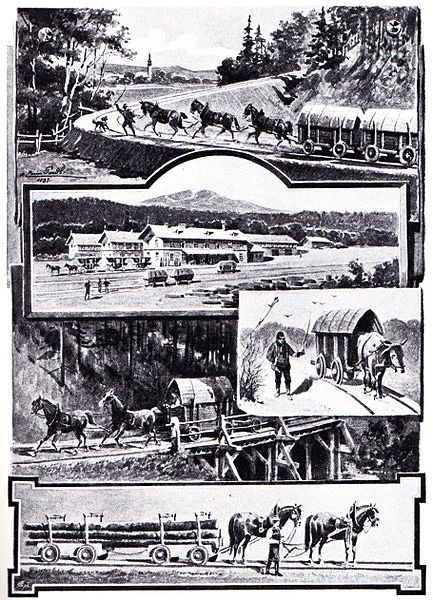
\includegraphics[height=0.5\paperheight]{geschichte/1787}
\note{%
Vorläufer im Bergbau
	1787 Ruhrkohle-Bergbau Pferdbahn, ein teil dieser schienen war aus Eisen - deshalb Eisenahn die andere aus Holz
}
\end{geschichte}

\begin{geschichte}
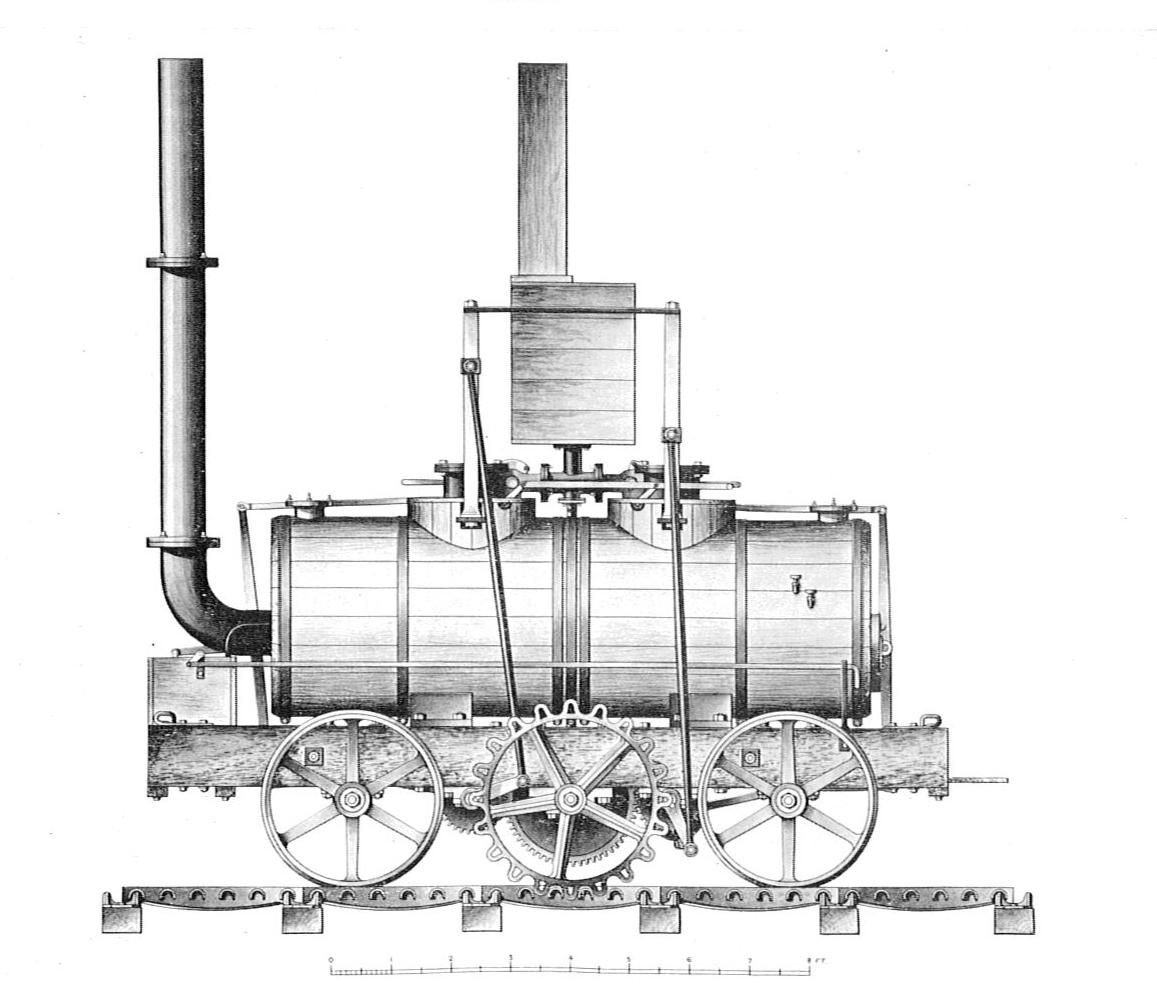
\includegraphics[height=0.5\paperheight]{geschichte/1815}
\note{%
	1815 Die Briten war erst, aber bereits in diesem Jahr hat Johann Friedrich Krigar eine Kopie von einem Britischen Model gebaut. Dann in 1818 eine weitere gebaut, aber es hat nicht die erwartende Leistung erfüllt
	Das erste Lokomotiv betriebene Eisenbahn in Deutschland war geoffnet am 1835:
	-Bilde von Ludwigsenbahn offnung
}
\end{geschichte}

\begin{geschichte}
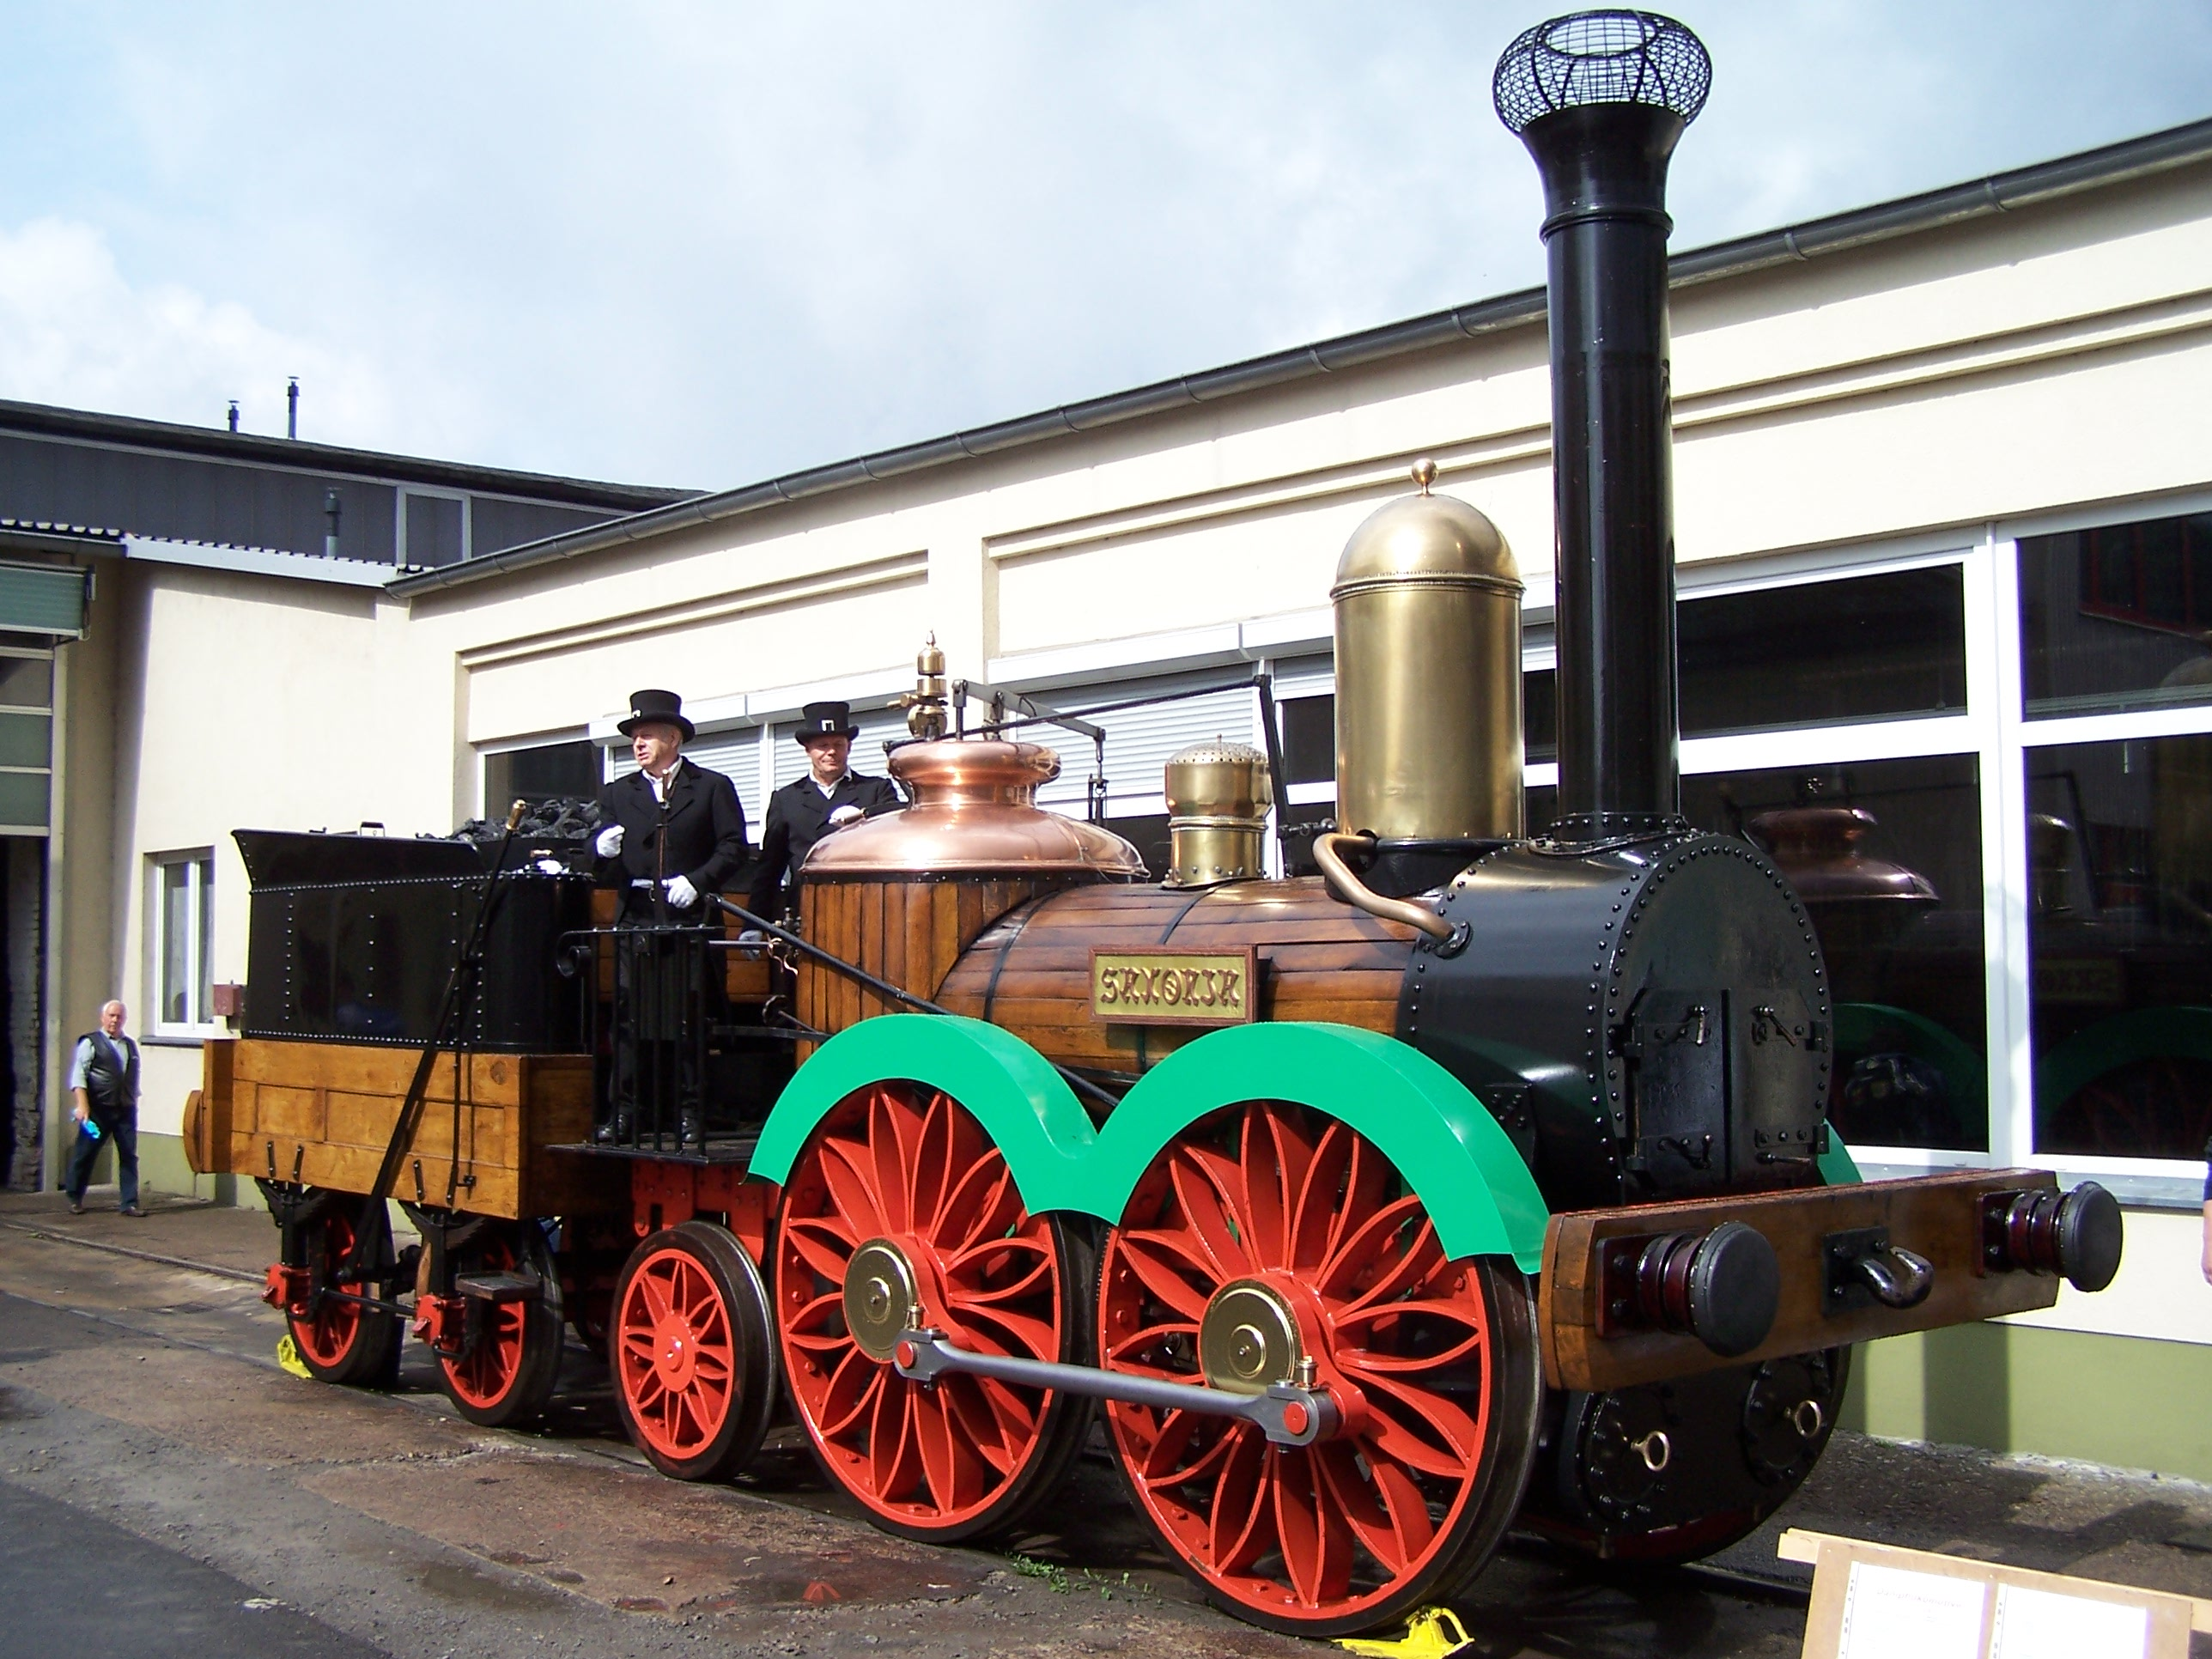
\includegraphics[height=0.5\paperheight]{geschichte/1839}
\note{%
	1836 erste Gütertransport, zwei Fässer Bier wurden in einem Fässer Bier wurden in einem Waggon der dritten Klasse transportiert
	1839 Umbau von zwei Personenwage zum regularen Gürtentransport. (vermutlich um mehr Bier zu transportier)
	Der Neubau von Eisenbahnstrecken erfolgte zuerst durch private Gesellschaften
	1839 in desalben Jahr auch bau der erste Fernverbindung zw. Leipzig und Dresden. Sachsen war der industriell starksten Region Deutschland damals Die damalige Geswindigkeit war maximal 35km-h Lokomotive Saxonia erst gebaute Deutsche lokomotive 115km in 3 Stunde
}
\end{geschichte}
\begin{geschichte}
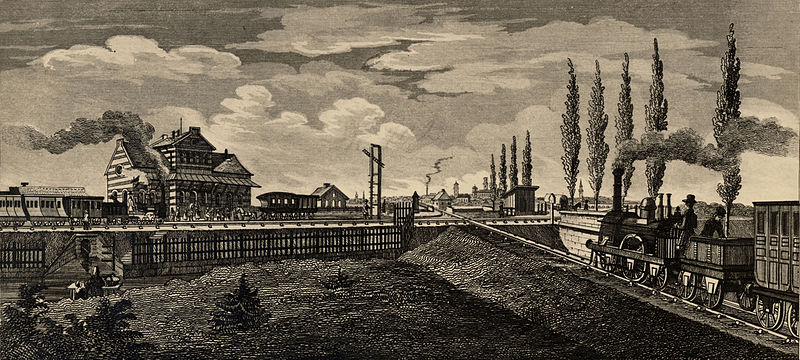
\includegraphics[height=0.4\paperheight]{geschichte/1845}
\note{%
	Further Kreuzung erste Umsteistation
}
\end{geschichte}
\begin{geschichte}
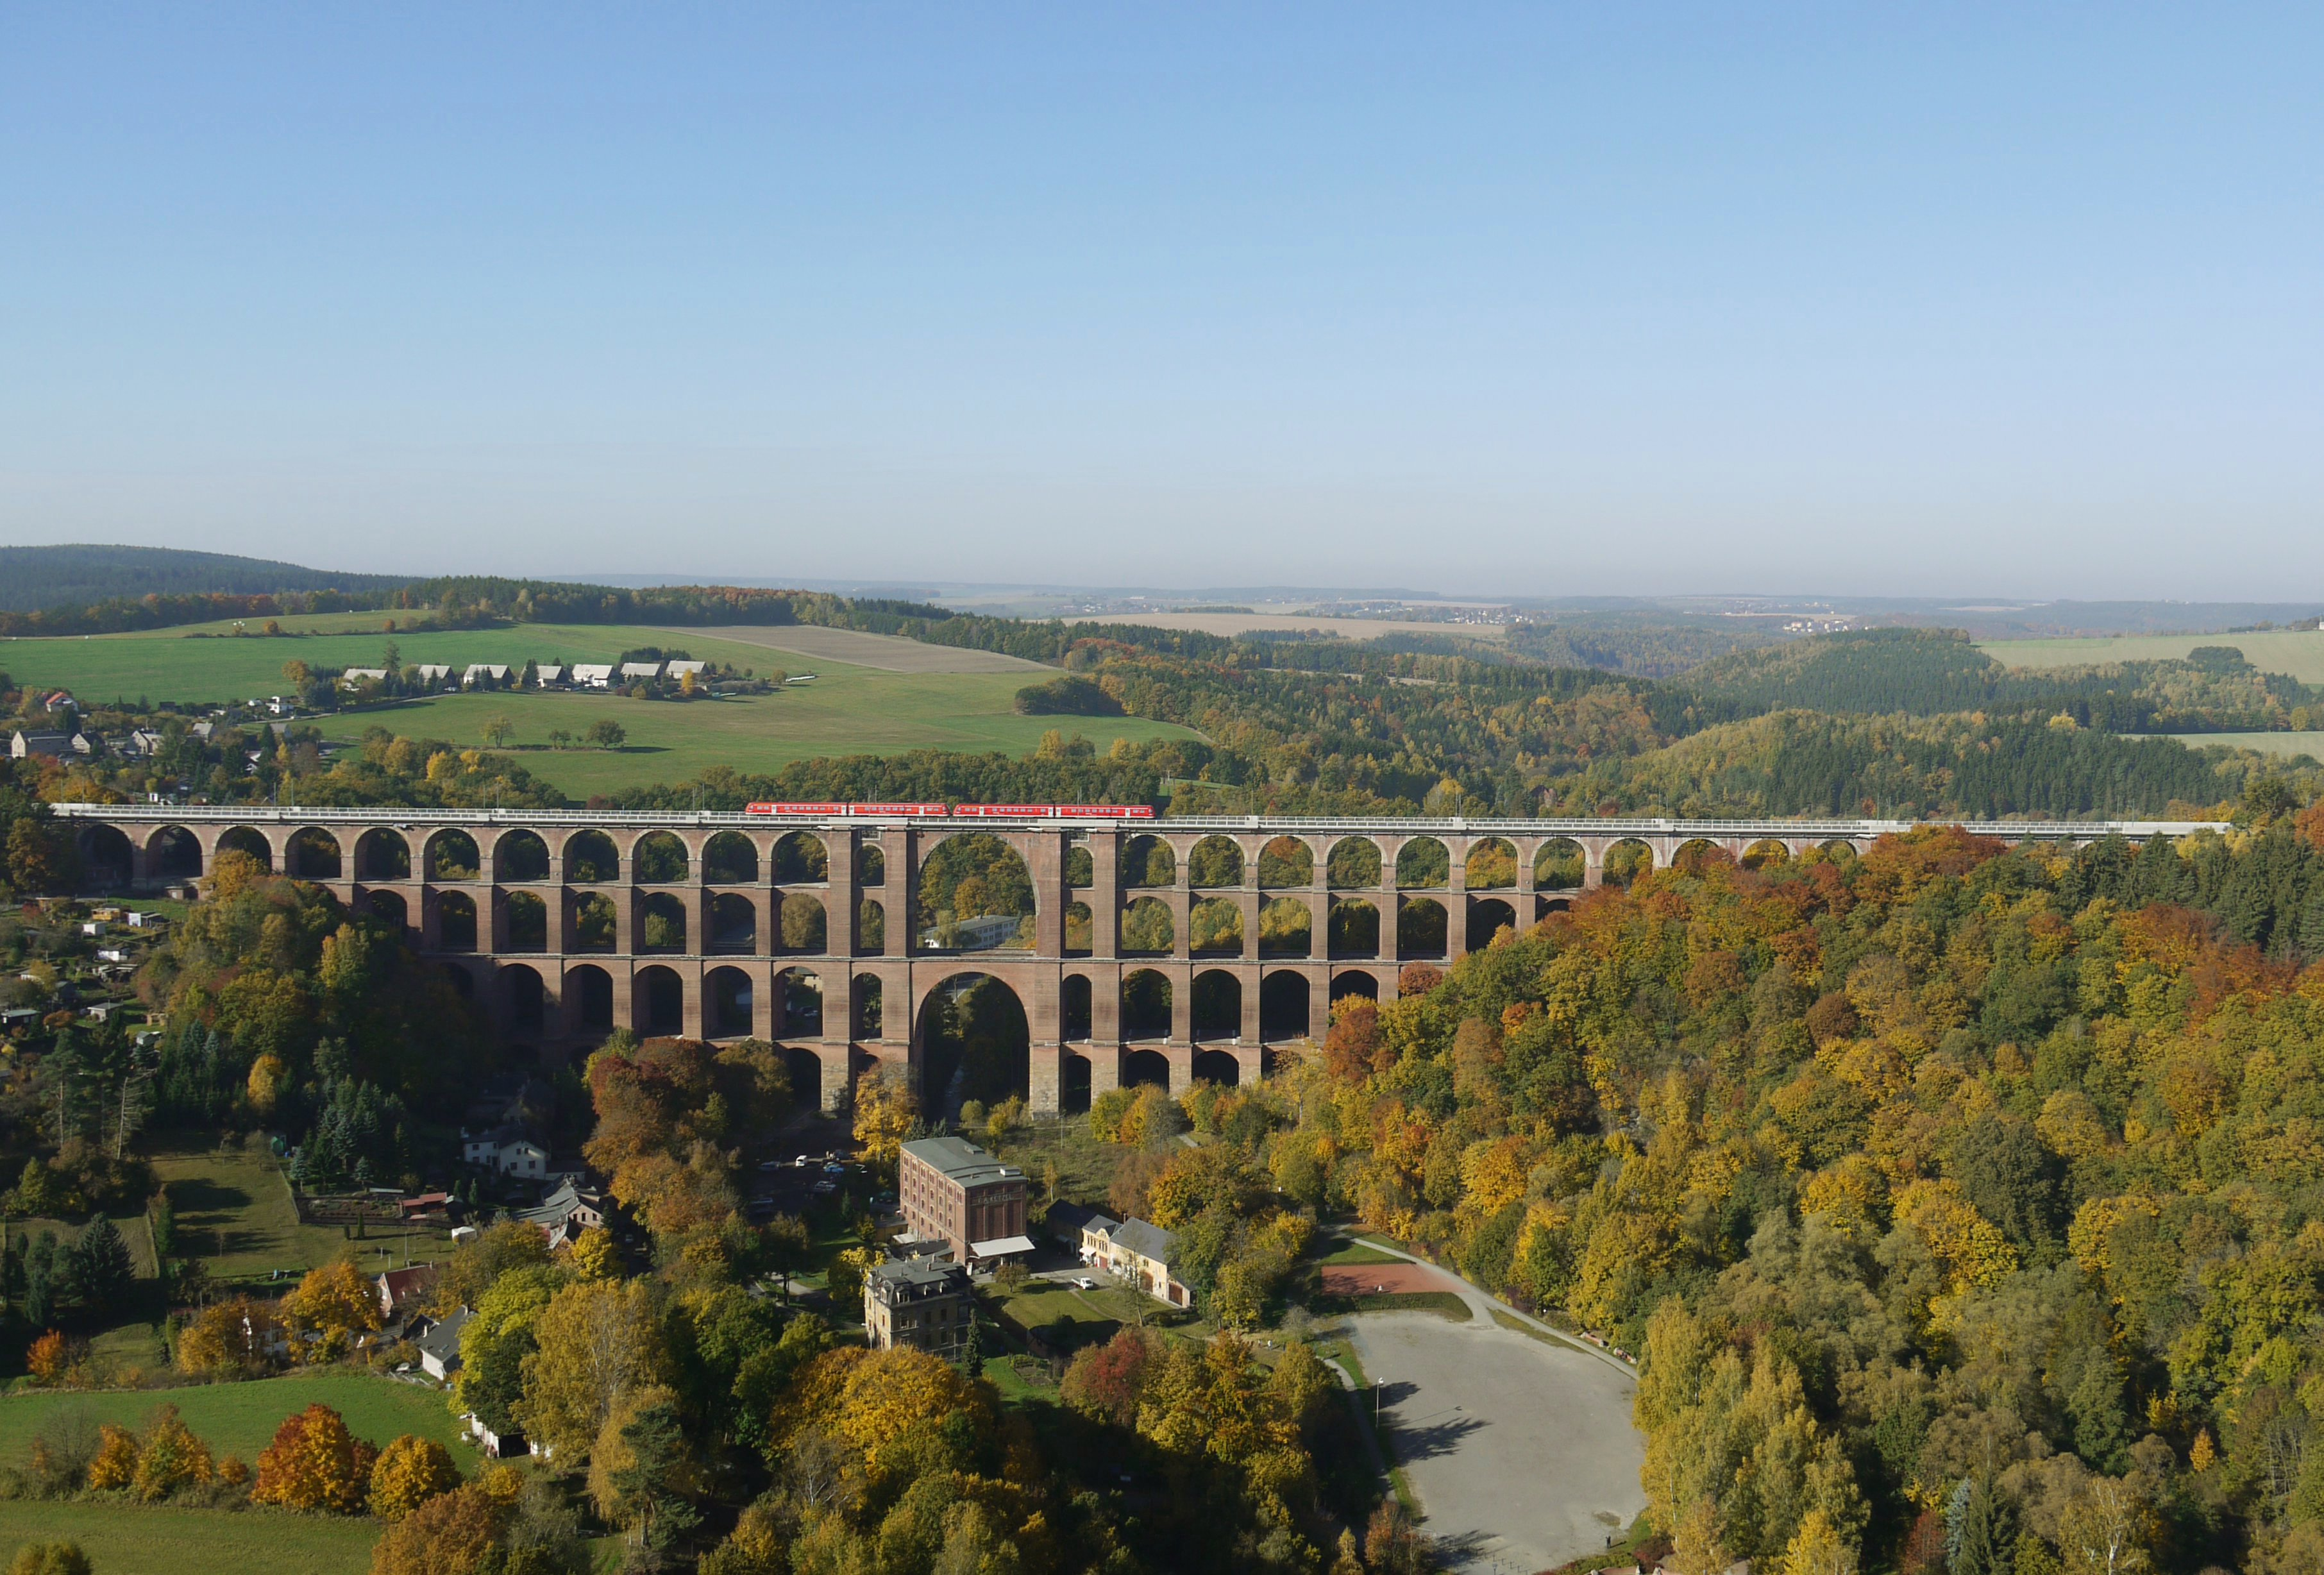
\includegraphics[height=0.5\paperheight]{geschichte/1851}
\note{%
	1851 Göltyschtalbrücke
	Nahverkehr
	Vor dem zweiten Weltkrieg waren die Deutscher großte Lokeexporteure der Welt. Es hat auch zu Sieg uber Frankreich geholfen in dieser Zeit
	Nach dem Ersten Weltkrieg im Weimarer Republik zunächst 1920 als Deutsche Reichseisenbahnen in der Verwaltung des Reiches
	Der Bahn wurde zu einem wichtigeren Teil des Staates

}
\end{geschichte}


\begin{geschichte}
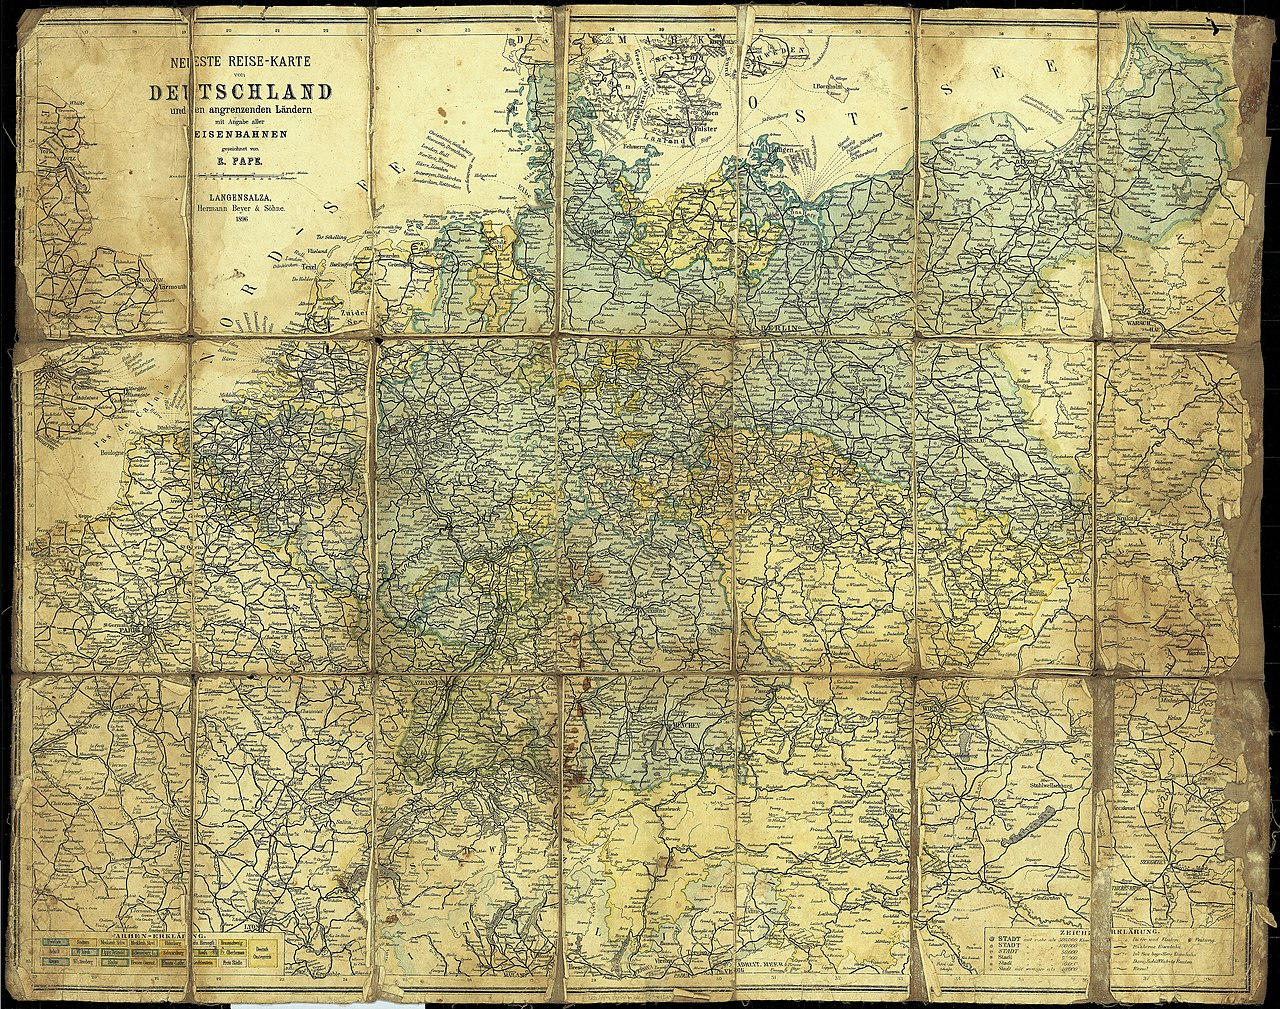
\includegraphics[height=0.5\paperheight]{geschichte/1871}
\note{
	1871 Staatsbahnen
	Bild ist aus 1896
	1924 zu einem einzigen Staatsunternehmen zusammen geschäft Reichsbahn-Gesellschaft den der größten Teil des Eisenbahnverkehrs in Deutschland übernahm
}
\end{geschichte}

\begin{geschichte}
\Large Deutschland war damals der größte Lokexporteur der WELT\\[4ex]
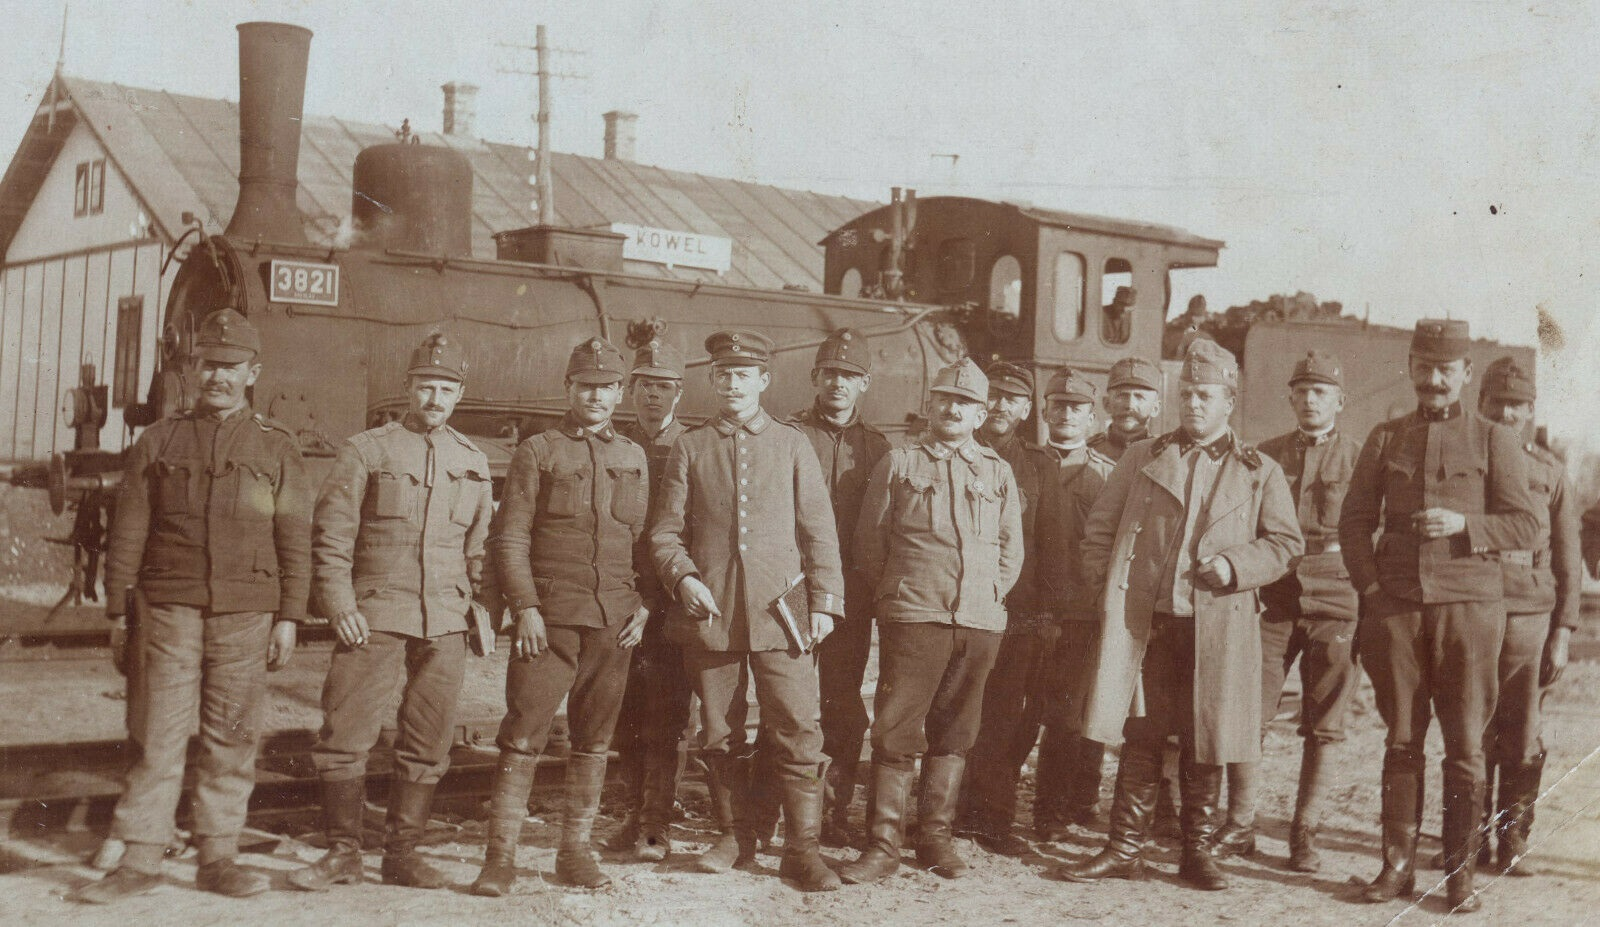
\includegraphics[height=0.4\paperheight]{geschichte/1914}
\end{geschichte}


\begin{geschichte}
\svg{10em}{geschichte/1924}
\note{%

	1949 Nach dem ende des zweiten Weltkrieges, Bundesrepublik Deutschland - Bundesbahn. Deutsche Demokratische Republik - Reichsbahn. Staatsbahnen
}
\end{geschichte}

\begin{geschichte}
\svg{10em}{geschichte/1949-1}
\hfill

\includegraphics[width=10em]{geschichte/1949-2}
\note{%
Erste Diesel Lokomotiven erschienen spater als die in der Sowjetunion nach dem ersten weltkrieg
}
\end{geschichte}

\begin{geschichte}
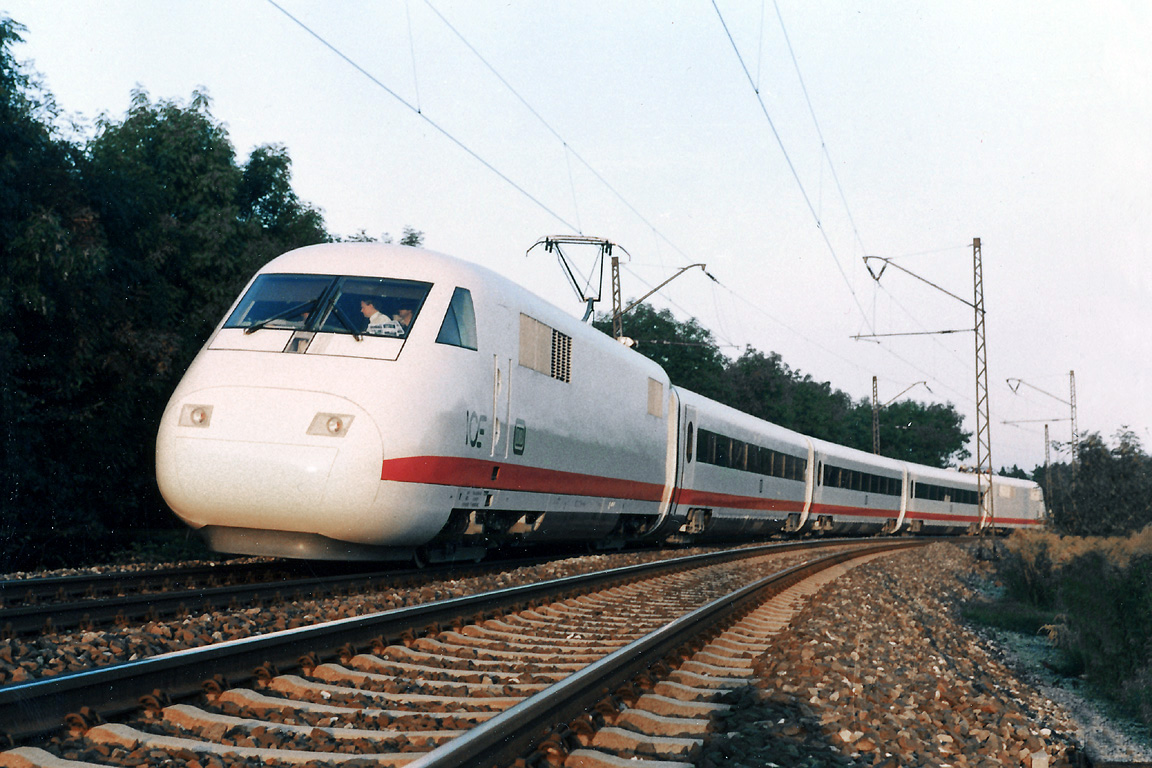
\includegraphics[height=.5\paperheight]{geschichte/1985}
\note{%
	1985 ICE-Vorläuferzug InterCityExperimental wurde im dieser Zeit ins Deinst gestellt
}
\end{geschichte}
\begin{geschichte}
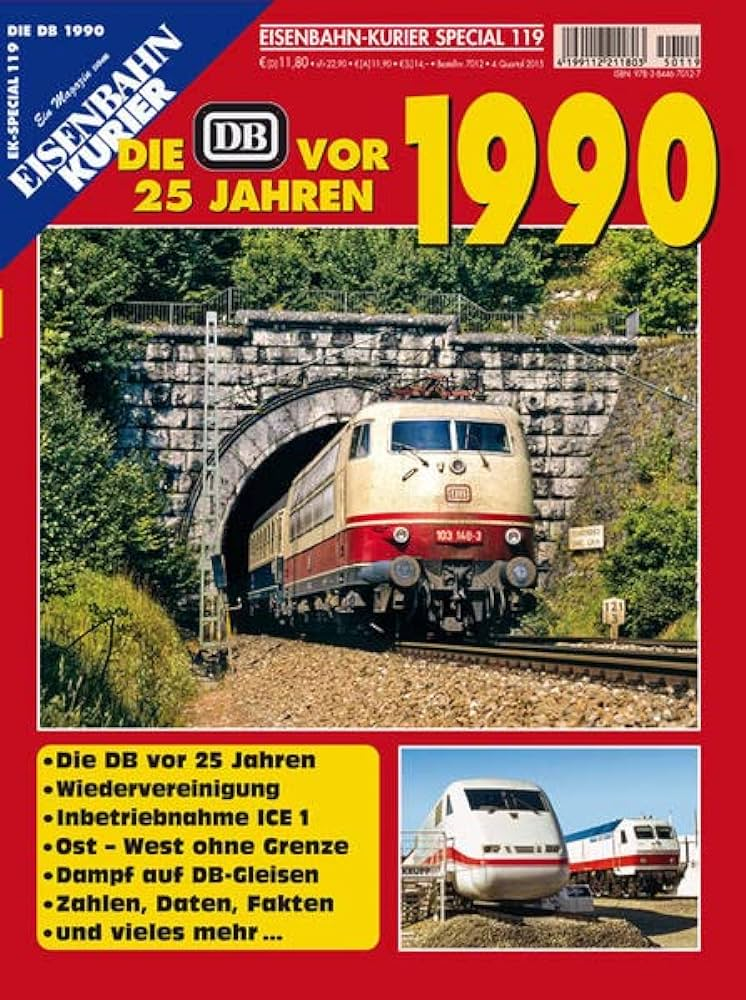
\includegraphics[height=.5\paperheight]{geschichte/1994}
\note{%
	in Schulden und das hat dazu gefurt das der Personal fast halbiert werden wurde, und viele Bahnofe wurden geschlossen. Dazu auch viele unrentable Strecken wurden geschlossen.
	-Regionalbahnofen sind ein zu uberwiegenden Last
	-Der Last war ausgeglichen mit andere Inkommensquellen

}
\end{geschichte}
